% !TEX spellcheck = en
\documentclass[main.tex]{subfiles} 

\begin{document}

\section{Results \& Interpretation}
\label{sec:5}

\subsection{Geodesic Solver}
\subsubsection{Sphere}
The transformation from spherical to cartesian coordinates is given as
\begin{align*}
    x &= u\sin(v)\cos(w)\\
    y &= u\sin(v)\sin(w)\\
    z &= u\cos(v)\\
\end{align*}

\begin{figure}[H]
\hspace{-20mm}\subfloat[$u'= 0,v'=0.2$.]{
	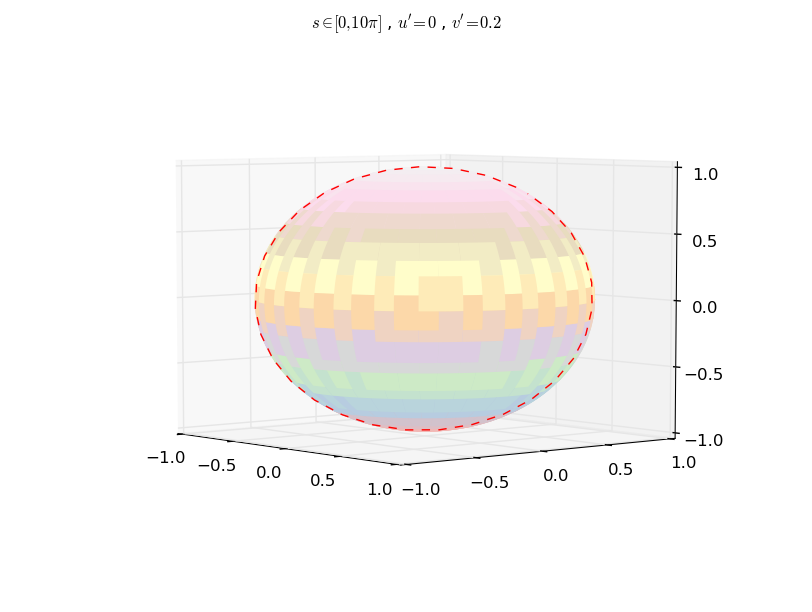
\includegraphics[scale=0.45,natwidth=812,natheight=612]
	{../figures/geodesic_curve_on_sphere3.png}}
\subfloat[$u'= 0.2,v'= 0$.]{
	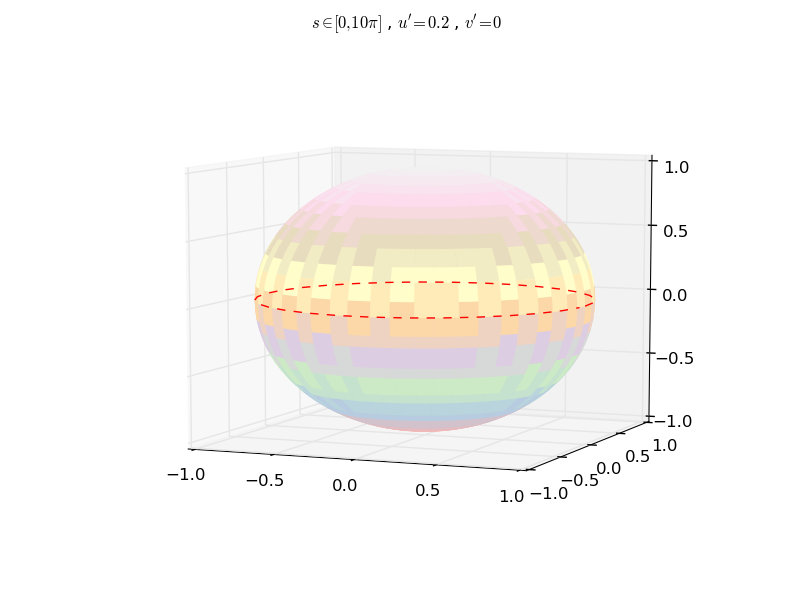
\includegraphics[scale=0.5,natwidth=812,natheight=612]
	{../figures/geodesic_curve_on_sphere5.png}}\\
\caption[Geodesic curves on a sphere]{Geodesic curves on a sphere}
\end{figure}

\begin{figure}[H]
\hspace{-20mm}\subfloat[$u'= 0,v'= 0.2$.]{
	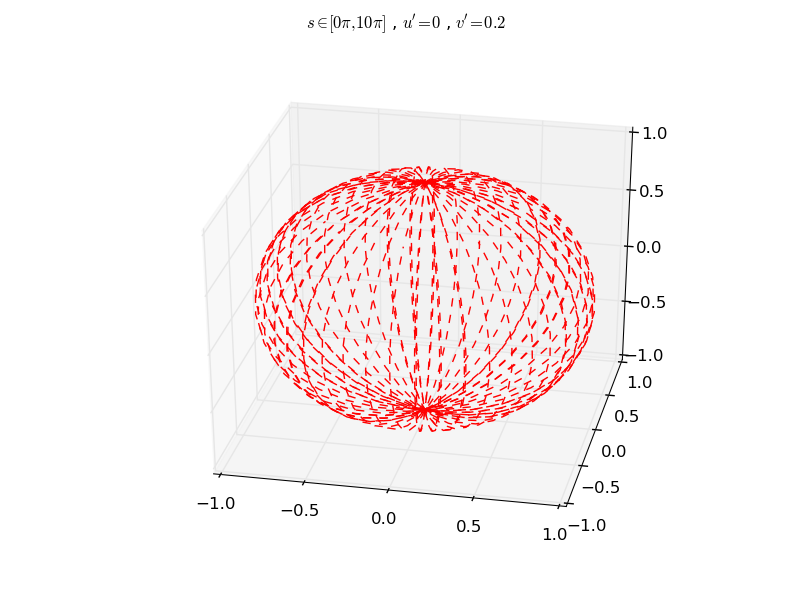
\includegraphics[scale=0.45,natwidth=812,natheight=612]
	{../figures/geodesic_curve_on_sphere4.png}}
\subfloat[$u'=0.1,v'=0.1$.]{
	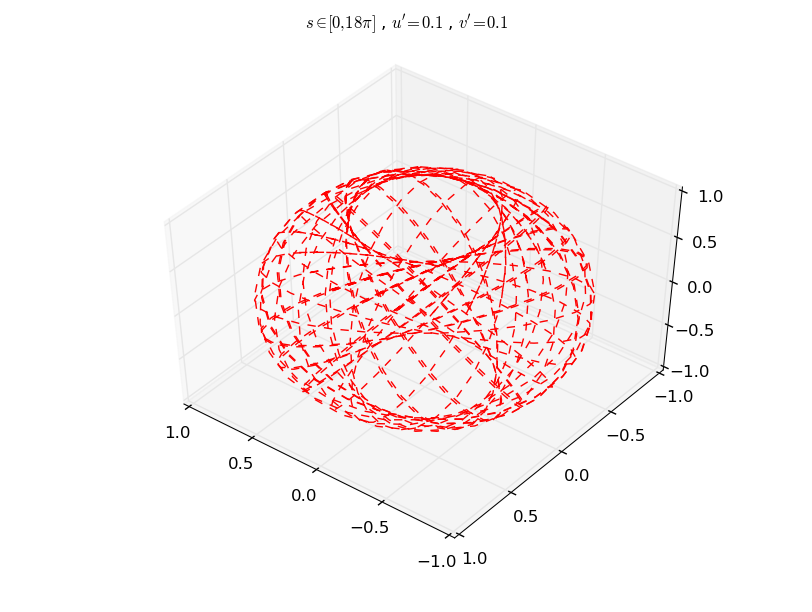
\includegraphics[scale=0.5,natwidth=812,natheight=612]
	{../figures/geodesic_curve_on_sphere2.png}}
\caption[Geodesic curves on a sphere.]{Geodesic curves on a sphere.}
\end{figure}


\subsubsection{Torus}
The transformation from toridal to cartesian coordinates is given as
\begin{align*}
	x &= (c + a\cos(u))\cos(v)\\
    y &= (c + a\cos(u))\sin(v)\\
    z &= \sin(u)\\
\end{align*}

\begin{figure}[H]
\hspace{-20mm}\subfloat[$u'=0.1,v'=.0$.]{
	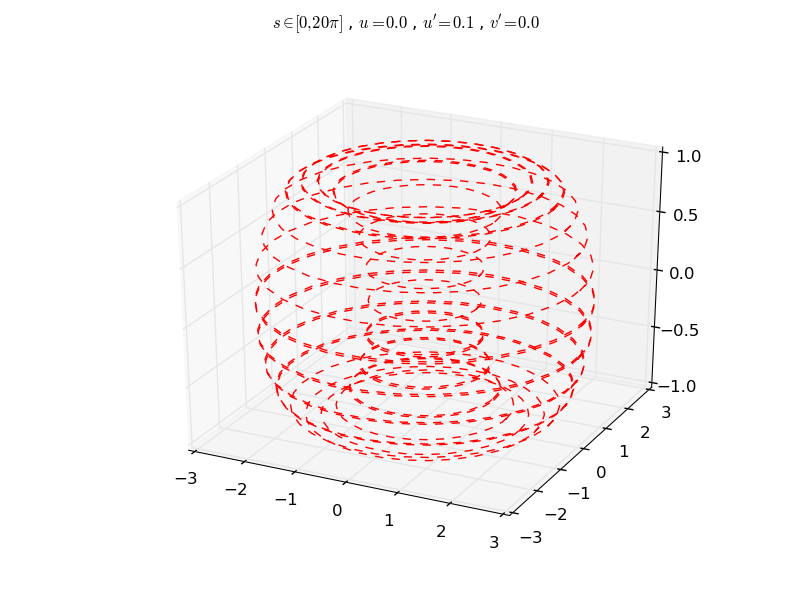
\includegraphics[scale=0.45,natwidth=812,natheight=612]
	{../figures/geodesic_curve_on_torus3.png}}
\subfloat[$u'=0,v'=0.1$.]{
	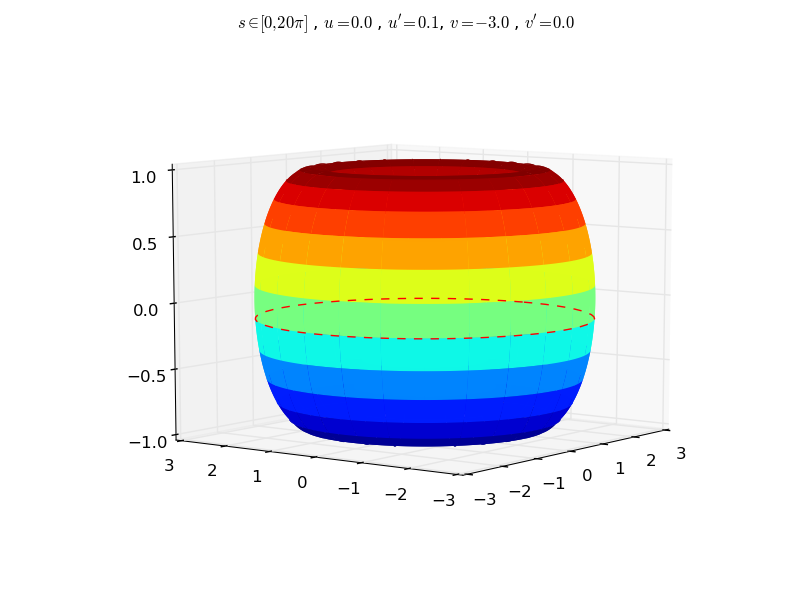
\includegraphics[scale=0.45,natwidth=812,natheight=612]
	{../figures/geodesic_curve_on_torus4.png}}
\hspace{-20mm}\subfloat[$u'=0.2,v'=0.2$.]{
	\hspace{25mm}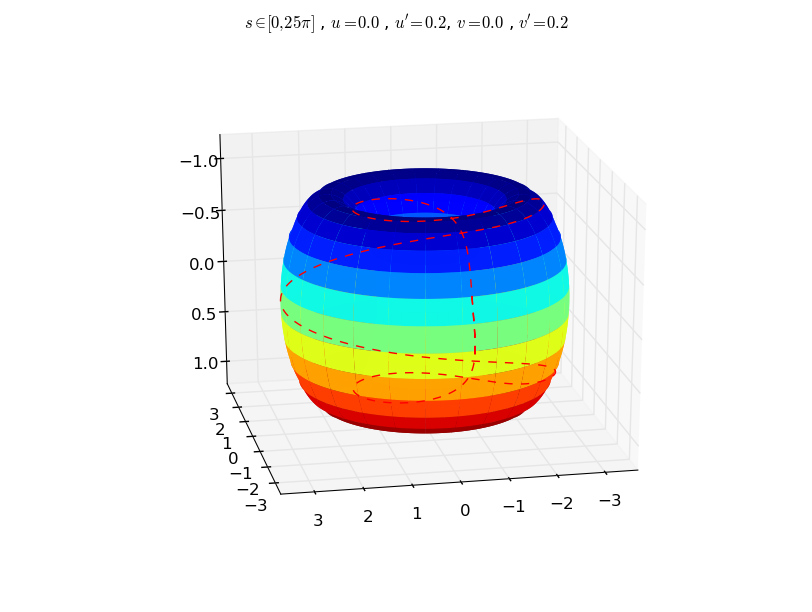
\includegraphics[scale=0.45,natwidth=812,natheight=612]
	{../figures/geodesic_curve_on_torus5.png}}
\caption[Geodesic curves on a torus.]{Geodesic curves on a torus.}
\end{figure}

\begin{figure}[H]
\hspace{-20mm}\subfloat[$u'=0.1,v'=0.1$.]{
	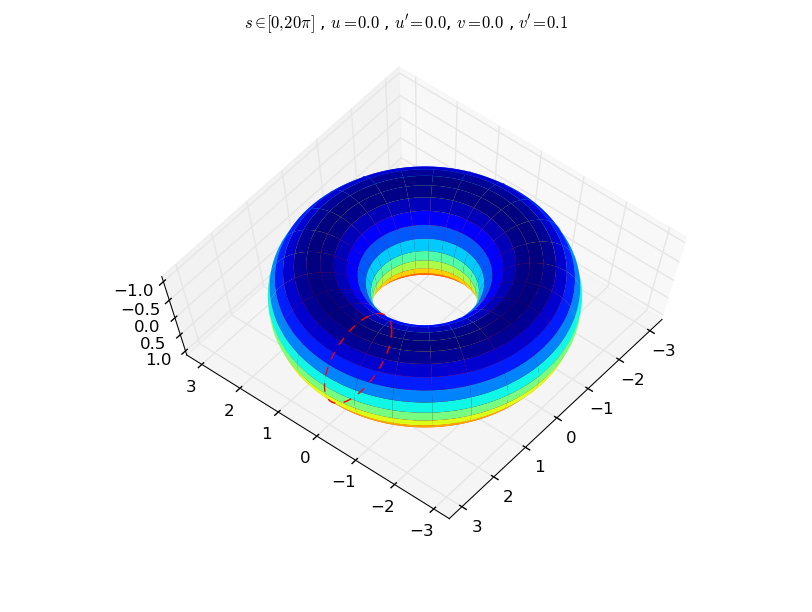
\includegraphics[scale=0.45,natwidth=812,natheight=612]
	{../figures/geodesic_curve_on_torus.png}}
	\subfloat[$u'=0.1,v'=0$.]{
	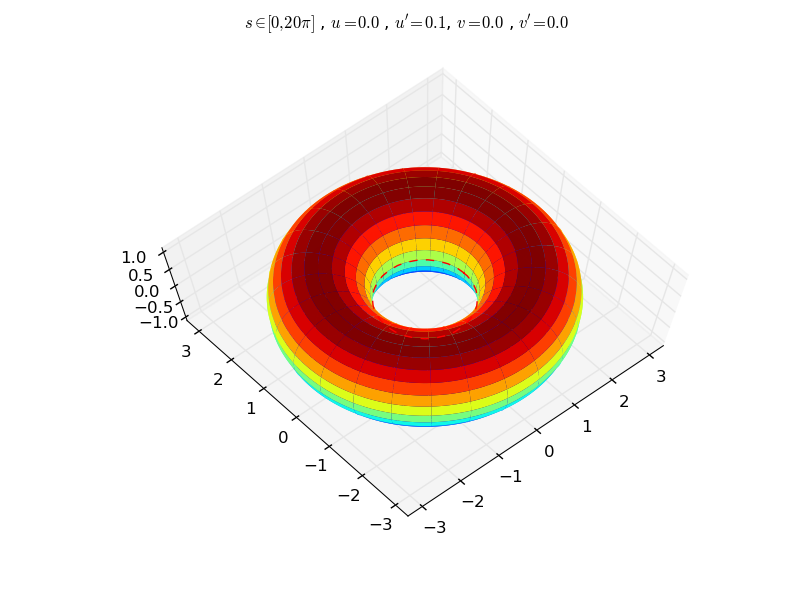
\includegraphics[scale=0.5,natwidth=812,natheight=612]
	{../figures/geodesic_curve_on_torus2.png}}
\caption[Geodesic curves on a torus.]{Geodesic curves on a torus.}
\end{figure}

\subsubsection{Cylindrical Catenoid}

\begin{align*}
    x &= \cos(u) - v\sin(u)\\
    y &= \sin(u) + v\cos(u)\\
    z &= v\\
\end{align*}


\begin{figure}[H]
\centering
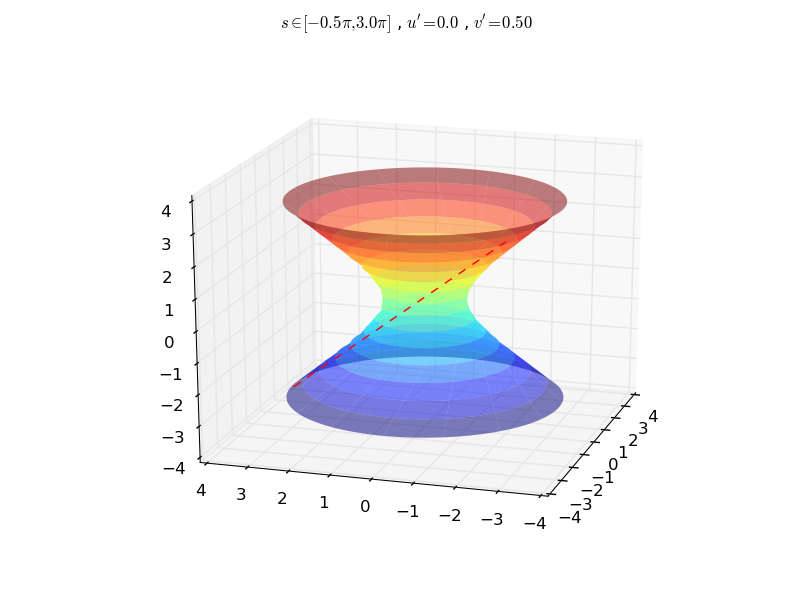
\includegraphics[scale=0.45,natwidth=812,natheight=612]
{../figures/geodesic_curve_on_catenoid.png}
\caption[Geodesic curves on a cylindrical catenoid.]{Geodesic curves on a cylindrical catenoid.}
\end{figure}


\subsubsection{Egg Carton Surface}

\begin{align*}
    x &= u\\
    y &= v\\
    z &= \sin(u)\cos(v)\\
\end{align*}

\begin{figure}[H]
\hspace{-20mm}\subfloat[$u'=0.1,v'=0.1$.]{
	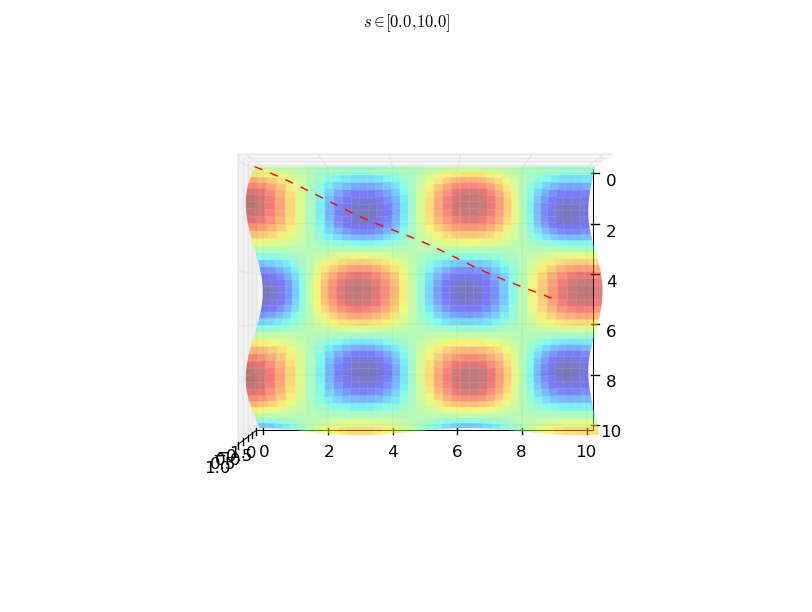
\includegraphics[scale=0.45,natwidth=812,natheight=612]
	{../figures/geodesic_curve_on_egg_carton.png}}
	\subfloat[$u'=0.1,v'=0.1$.]{
	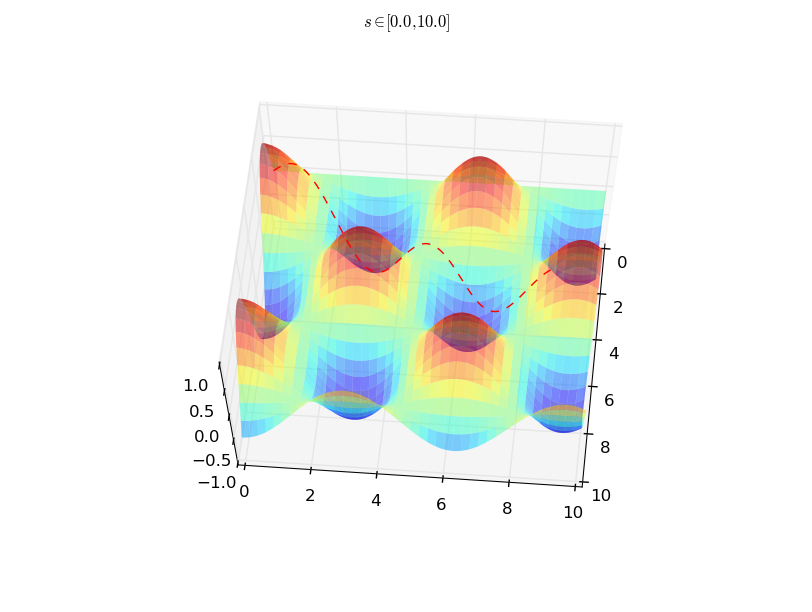
\includegraphics[scale=0.45,natwidth=812,natheight=612]
	{../figures/geodesic_curve_on_egg_carton2.png}}
\caption[Geodesic curves on an egg carton surface.]{Geodesic curves on an egg carton surface.}
\end{figure}


\subsubsection{Mobius Strip}

\begin{align*}
	x &= \left[1 + \frac{v}{2}\cos\left(\frac{u}{2}\right)\right]\cos\left(u\right)\\
    y &= \left[1 + \frac{v}{2}\cos\left(\frac{u}{2}\right)\right]\sin\left(u\right)\\
    z &= \frac{v}{2}\sin\left(\frac{u}{2}\right)\\
\end{align*}

\begin{figure}[H]
\centering
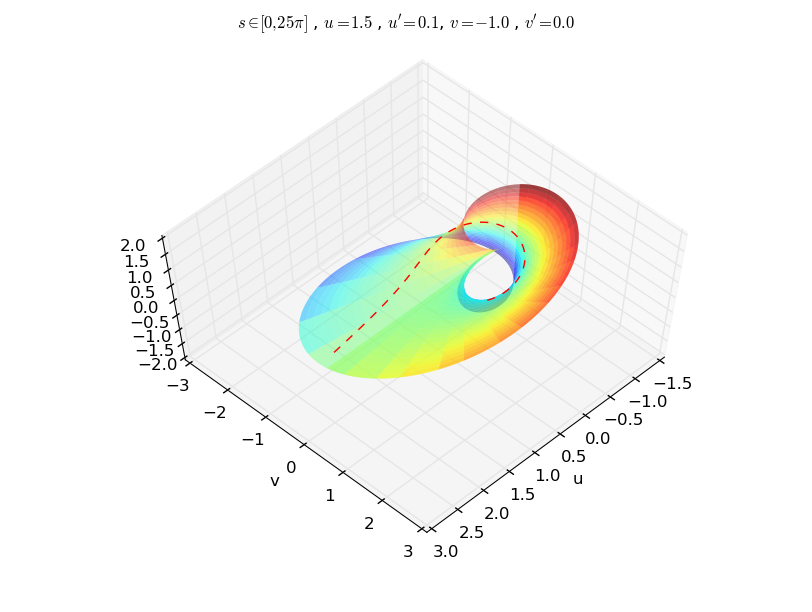
\includegraphics[scale=0.45,natwidth=812,natheight=612]
{../figures/geodesic_curve_on_mobius_strip.png}
\caption[Geodesic curve on a Mobius strip.]{Geodesic curve on a Mobius strip.}
\end{figure}

\subsubsection{3D Kerr Metric}

The Kerr metric is given as
\begin{align*}
ds^2 = &-\left(1 - \frac{2GMr}{r^2+a^2\cos^2(\theta)}\right) dt^2 +
	      \left(\frac{r^2+a^2\cos^2(\theta)}{r^2-2GMr+a^2}\right) dr^2 +
		  \left(r^2+a^2\cos(\theta)\right) d\theta^2\\ 
		&+
		  \left(r^2+a^2+\frac{2GMra^2}{r^2+a^2\cos^2(\theta)}\right)\sin^2(\theta) d\phi^2 -
		  \left(\frac{4GMra\sin^2(\theta)}{r^2+a^2\cos^2(\theta)}\right) d\phi\, dt
\end{align*}
For $a = 0$, this reduces to the Schwarzchild metric. We have run the geodesic solver
for this case, and used the Schwarzchild radius to determine a relationship between 
the coeffiencts G and M, which amounts to determining the geodesics near a black hole.

\begin{figure}[H]
\hspace{-20mm}{
	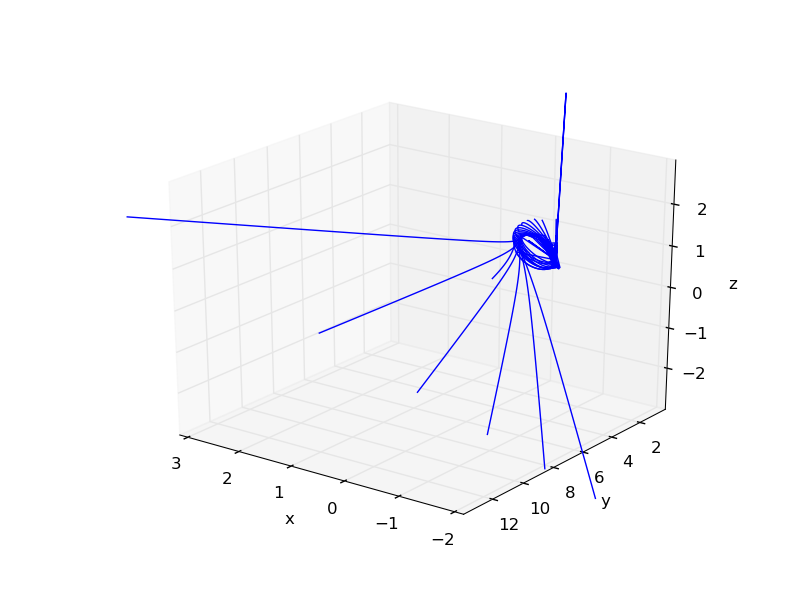
\includegraphics[scale=0.45,natwidth=812,natheight=612]
	{../figures/geodesic_curve_for_3d_kerr_metric3.png}} 
	{
	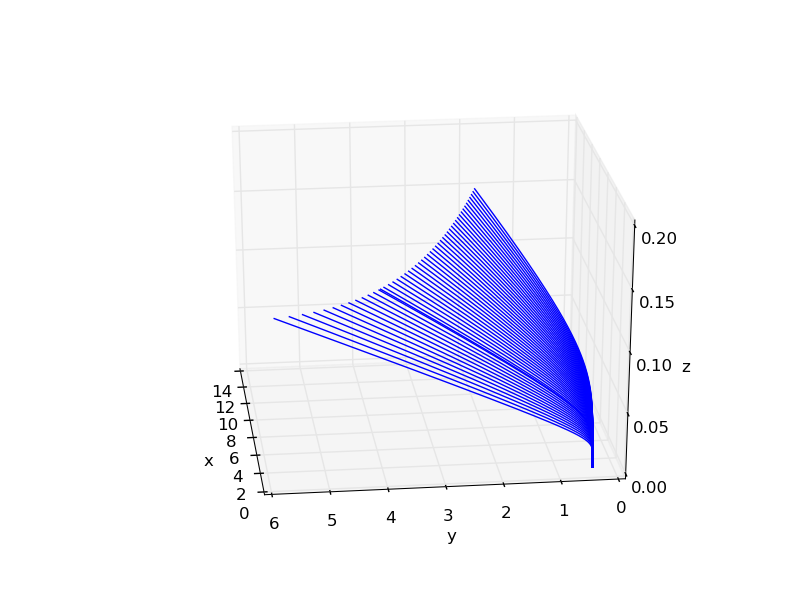
\includegraphics[scale=0.45,natwidth=812,natheight=612]
	{../figures/geodesic_curve_for_3d_kerr_metric4.png}}
\caption[Geodesic curves near a black hole.]{Geodesic curves near a black hole.}
\end{figure}

\end{document}